%!TEX program = lualatex
\documentclass[12pt]{article}
\usepackage[
  margin=1.5cm,
  includefoot,
  footskip=10pt,
]{geometry}

\usepackage{unicode-math}
\setmathfont{Cambria Math}
\setmainfont{Cambria}
%\usepackage{amsmath}
\usepackage{multicol}
\usepackage{graphicx}
%\usepackage{fullpage}
\usepackage[
  margin=1.5cm,
  includefoot,
  footskip=10pt,
]{geometry}
\pagestyle{empty}
\usepackage{subfig}
\begin{document}
{\centering\Large Basic Chords (v0.1)\par}\medskip

\begin{figure}[!h]%
    \centering
    \subfloat{{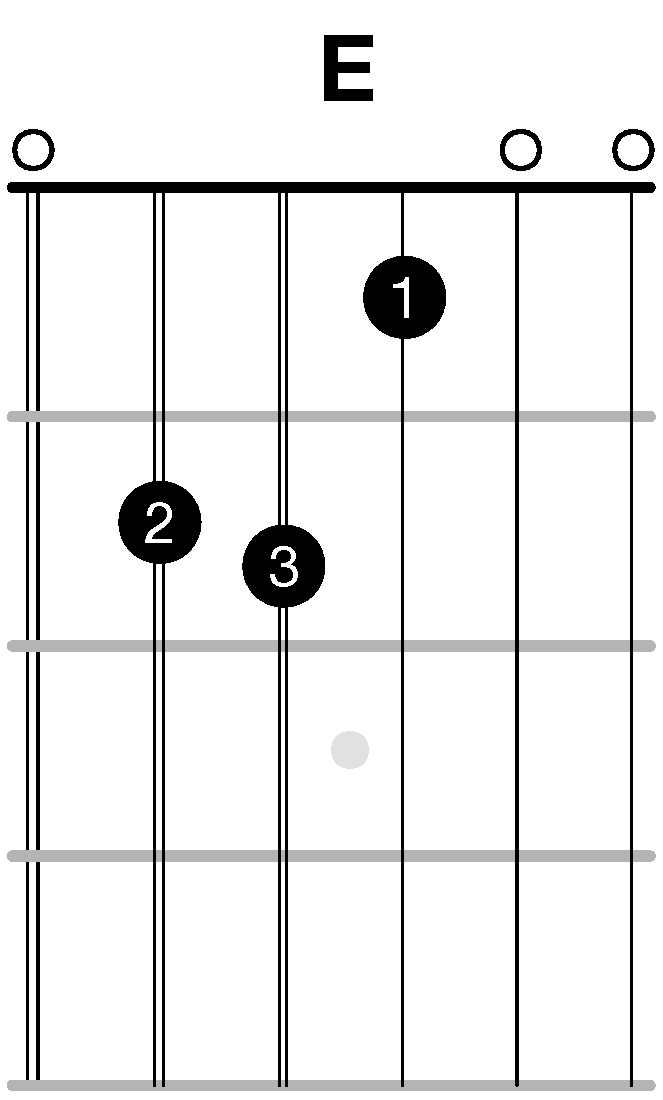
\includegraphics[width=3cm]{chords/E.pdf} }}%
    \quad
    \subfloat{{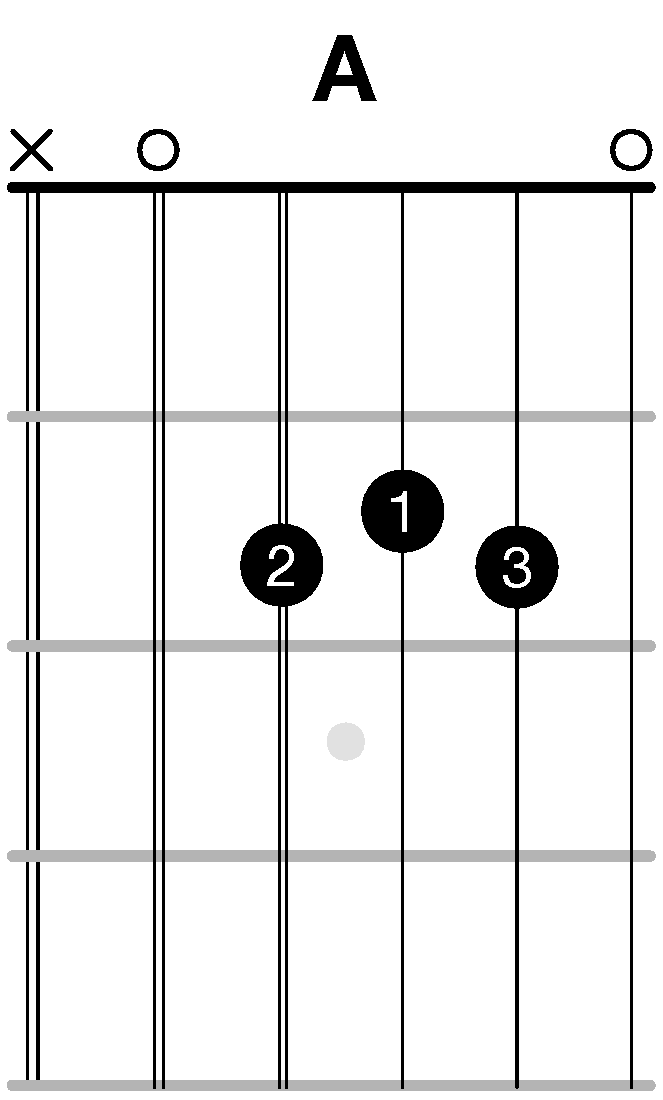
\includegraphics[width=3cm]{chords/A.pdf} }}%
    \quad
    \subfloat{{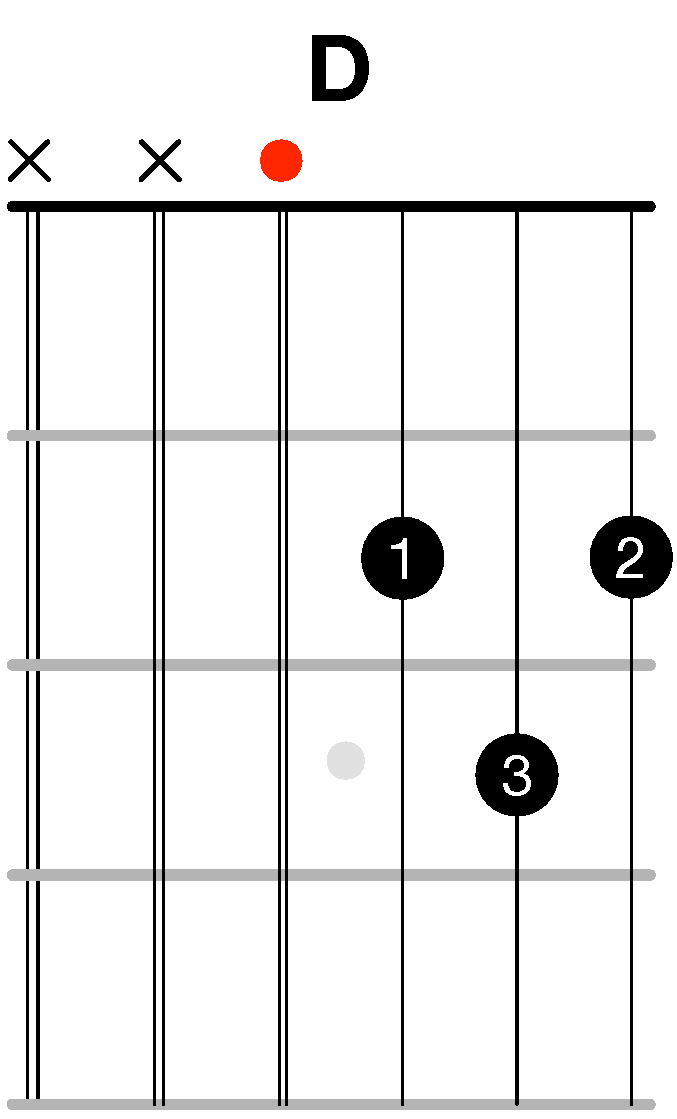
\includegraphics[width=3cm]{chords/D.pdf} }}%
    \quad
    \subfloat{{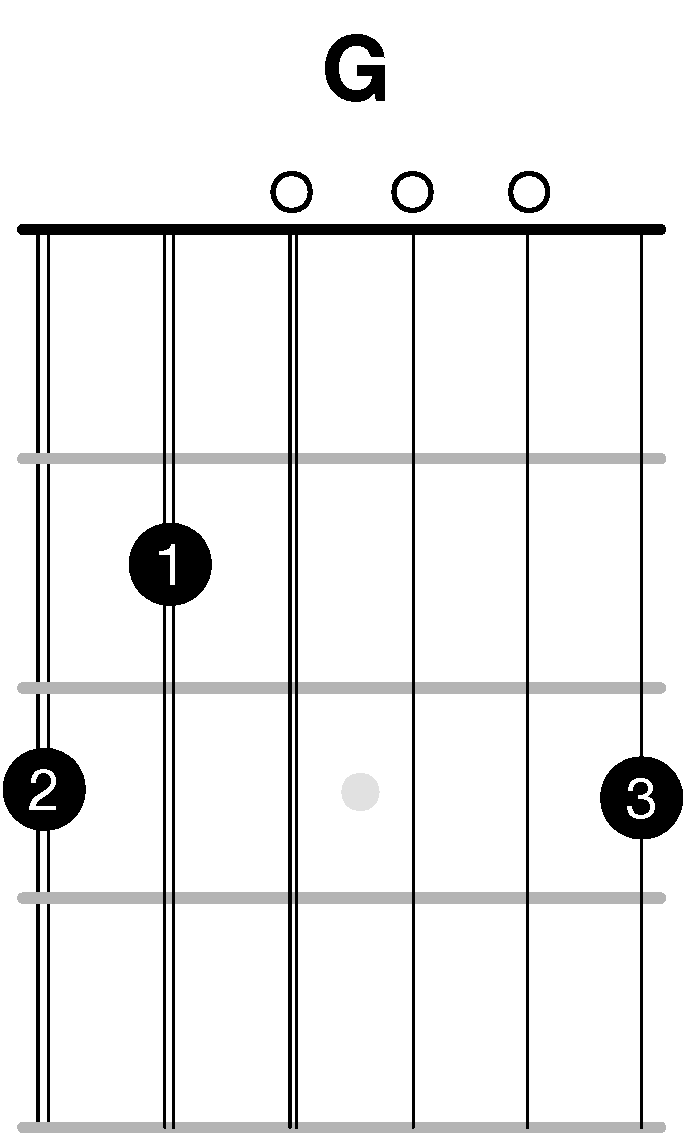
\includegraphics[width=3cm]{chords/G.pdf} }}%
    \quad
    \subfloat{{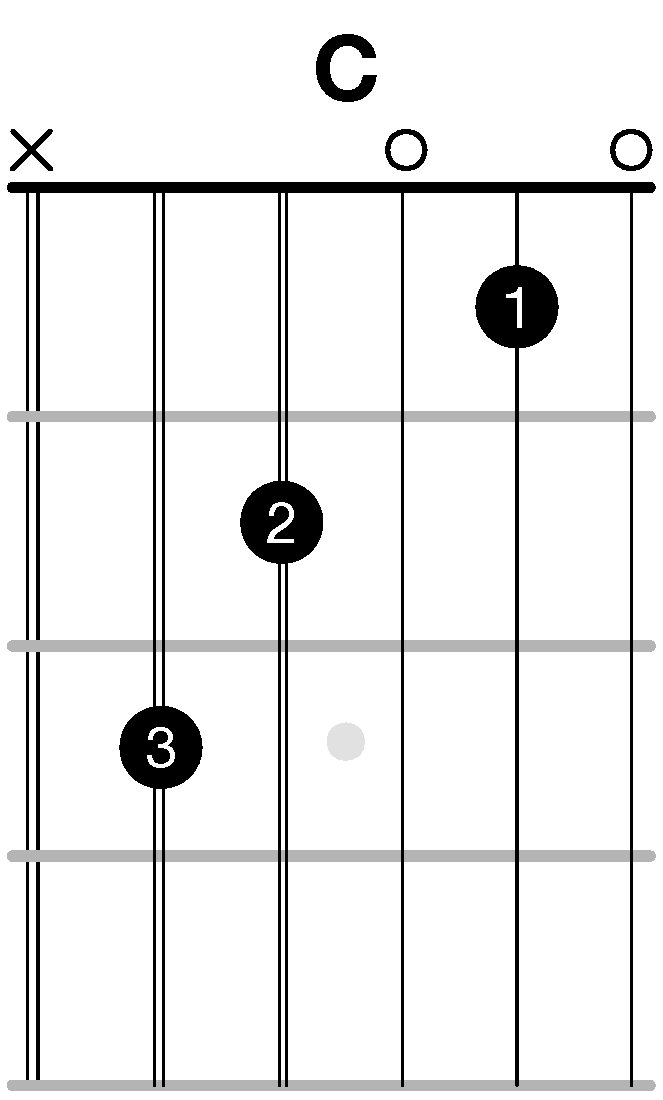
\includegraphics[width=3cm]{chords/C.pdf} }}%
    \vspace{1cm}
    \subfloat{{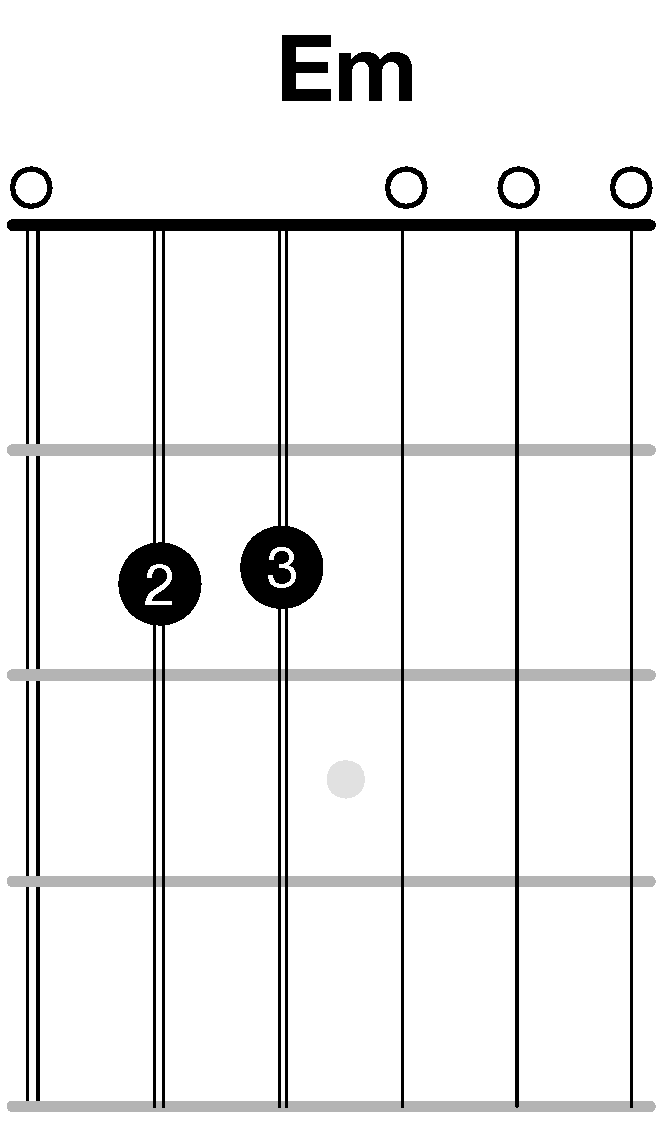
\includegraphics[width=3cm]{chords/Em.pdf} }}%
    \quad
    \subfloat{{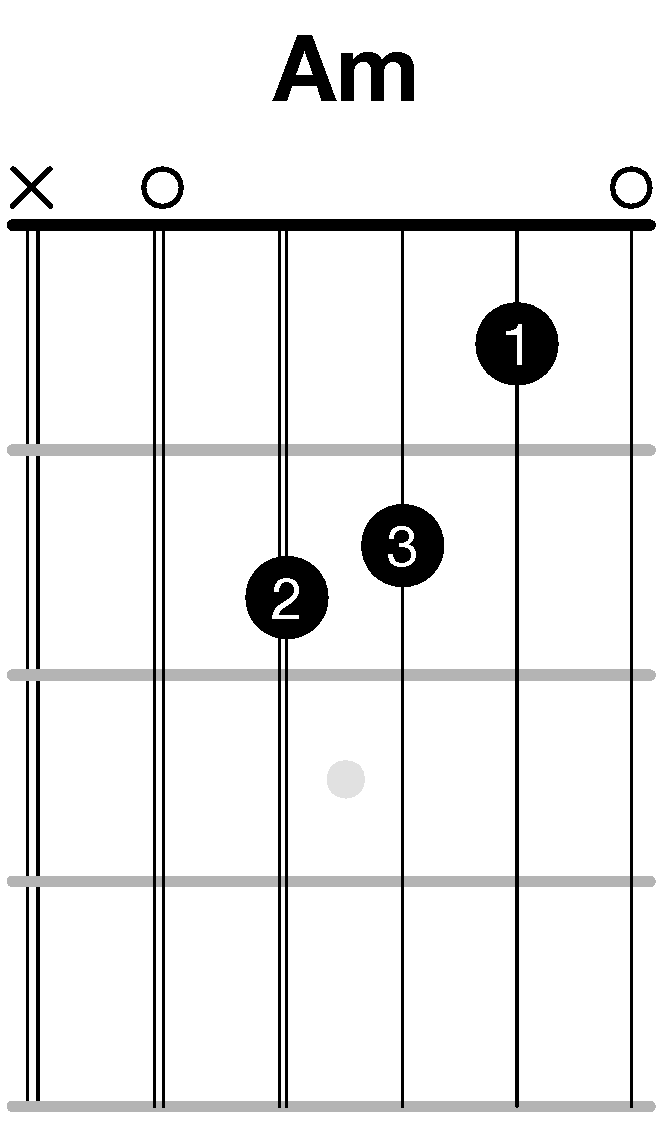
\includegraphics[width=3cm]{chords/Am.pdf} }}%
    \quad
    \subfloat{{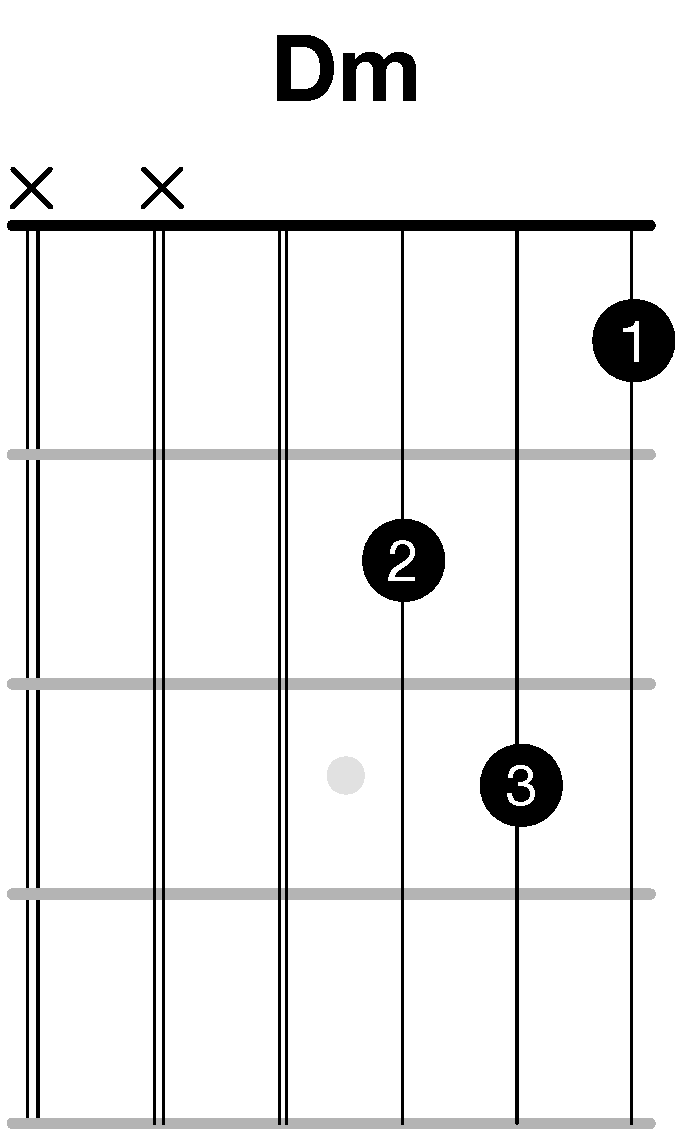
\includegraphics[width=3cm]{chords/Dm.pdf} }}%
    \quad
    \subfloat{{
\includegraphics[width=3cm]{chords/blank.pdf} }}%
    \quad
    \subfloat{{
\includegraphics[width=3cm]{chords/blank.pdf} }}%
    \vspace{1cm}
    \subfloat{{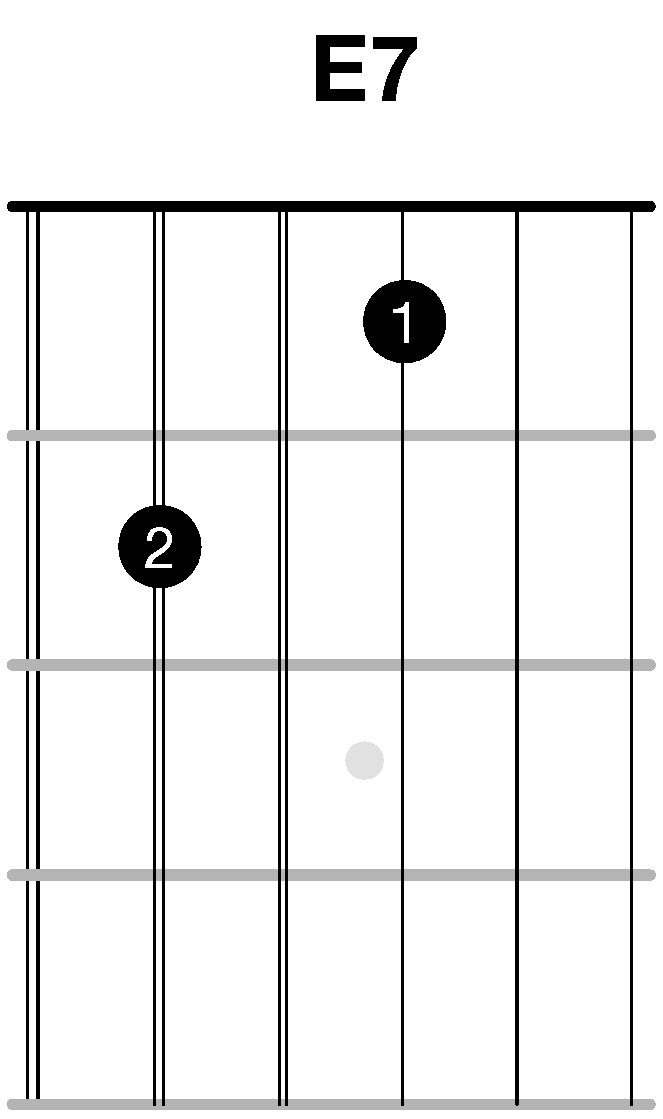
\includegraphics[width=3cm]{chords/E7.pdf} }}%
    \quad
    \subfloat{{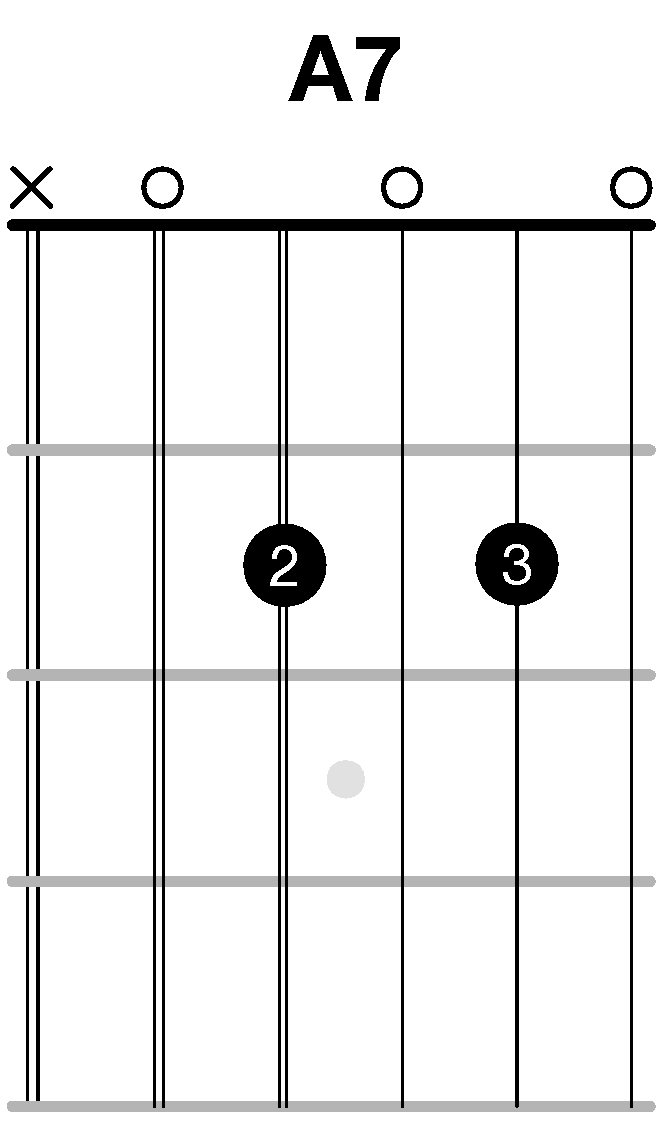
\includegraphics[width=3cm]{chords/A7.pdf} }}%
    \quad
    \subfloat{{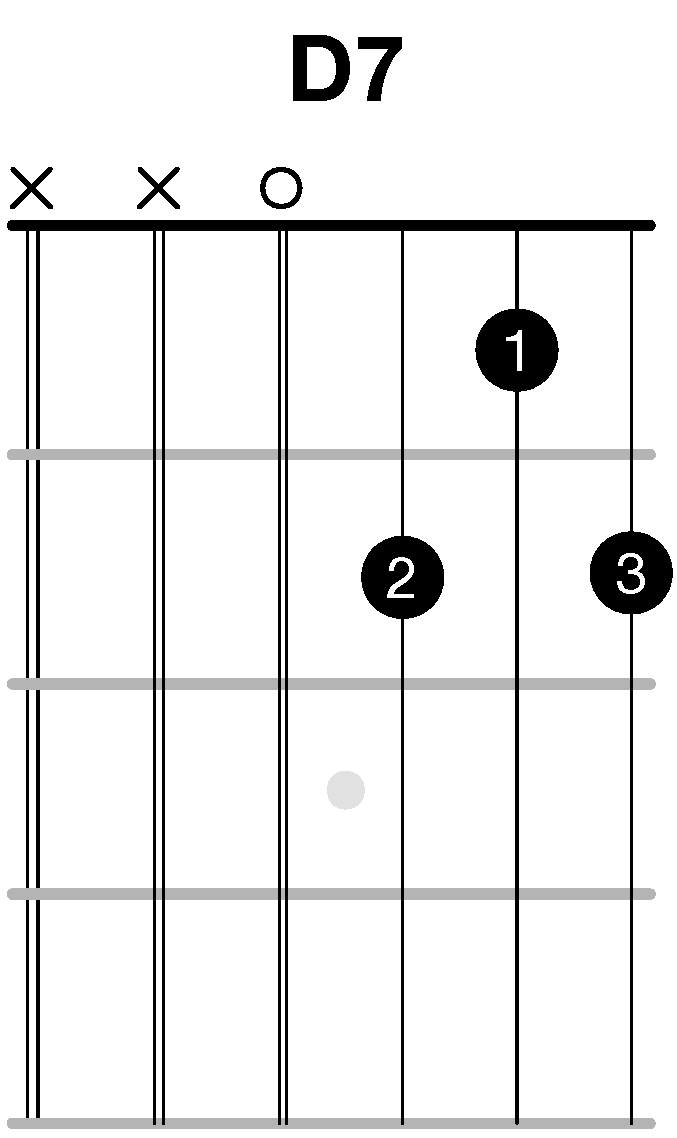
\includegraphics[width=3cm]{chords/D7.pdf} }}%
    \quad
    \subfloat{{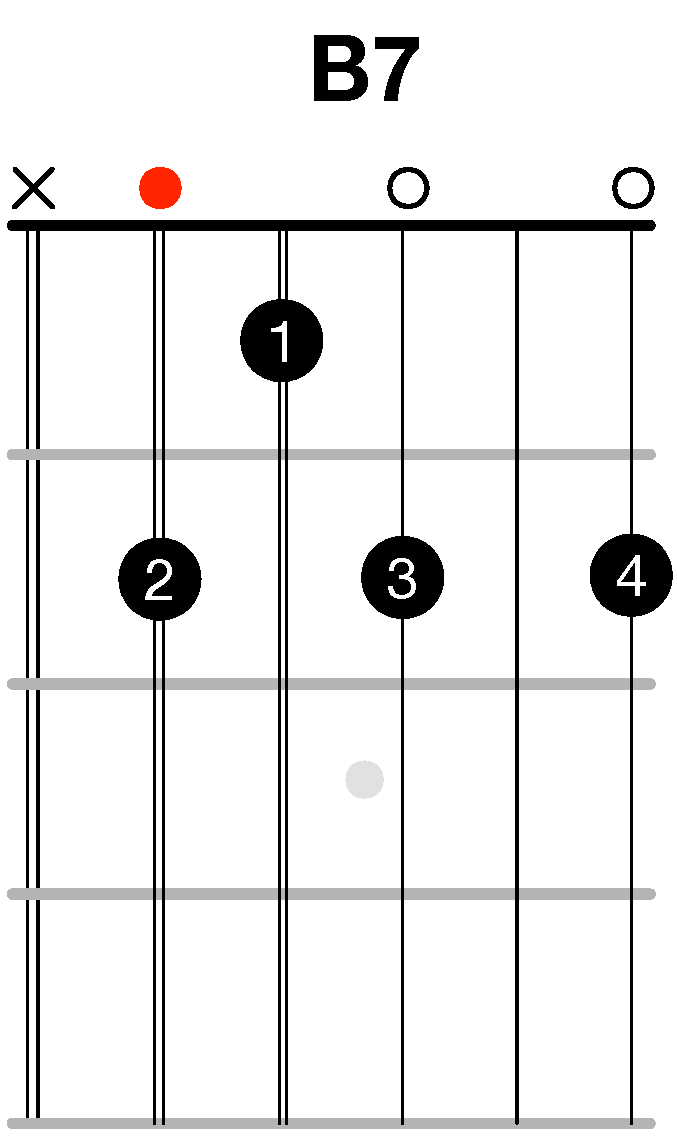
\includegraphics[width=3cm]{chords/B7.pdf} }}%
    \quad
    \subfloat{{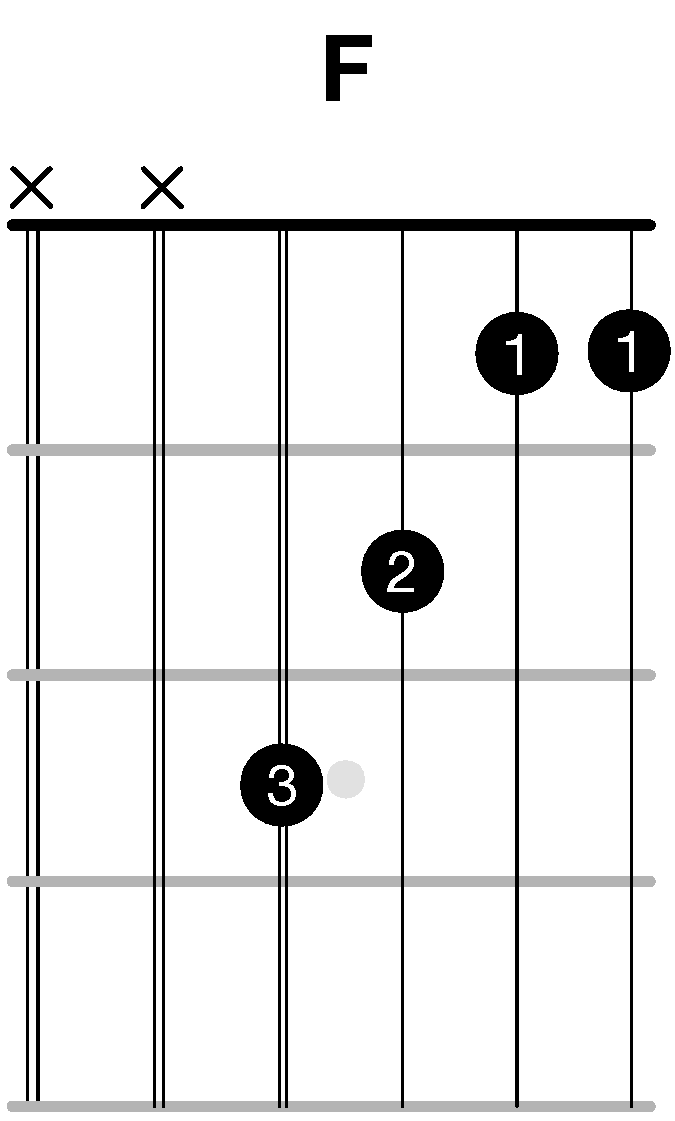
\includegraphics[width=3cm]{chords/F.pdf} }}%

  \end{figure}
\end{document}
